\documentclass[10pt]{article}
\usepackage[a4paper, margin=2.3cm]{geometry}
\usepackage{titlesec}
\usepackage{graphicx}
\usepackage{subcaption}
\usepackage{booktabs}
\usepackage{amsmath}
\usepackage{hyperref}
\usepackage{enumitem}
\usepackage{parskip}
\usepackage{xcolor}
\usepackage{ulem}
\usepackage{float}
\usepackage{placeins}
\usepackage{tikz}
\usepackage{caption}
\usetikzlibrary{arrows.meta}

% Compact formatting to keep the report within the 8-page limit
\linespread{0.98}
\setlength{\textfloatsep}{8pt plus 2pt minus 2pt}
\setlength{\floatsep}{6pt plus 2pt minus 2pt}
\setlength{\intextsep}{6pt plus 2pt minus 2pt}
\setlength{\abovecaptionskip}{4pt}
\setlength{\belowcaptionskip}{2pt}
\setlength{\parskip}{3pt}
\definecolor{figBlue}{HTML}{2563EB}
\definecolor{figGreen}{HTML}{16A34A}
\definecolor{figAmber}{HTML}{D97706}
\definecolor{figPink}{HTML}{DB2777}
\definecolor{figIndigo}{HTML}{4F46E5}
\definecolor{figCyan}{HTML}{0284C7}
\definecolor{figOrange}{HTML}{EA580C}
\definecolor{figRed}{HTML}{DC2626}
\definecolor{figOlive}{HTML}{65A30D}
\captionsetup{font=small}

\title{COMP3242 Group Project Report\\Ablation Study of SimCLR Components}

\titleformat{\section}
  {\normalfont\large\bfseries}
  {\thesection}
  {0.8em}
  {}

\titleformat{\subsection}
  {\normalfont\normalsize\bfseries}
  {\thesubsection}
  {0.8em}
  {}

\titlespacing*{\section}{0pt}{8pt}{8pt}
\titlespacing*{\subsection}{0pt}{8pt}{8pt}

\author{
Chengbo Yan \\ \texttt{u7515796}
\and
Guochen Wang \\ \texttt{u7663394}
\and
Weiyi Jiang \\ \texttt{u8191809}
}

\date{June 2026}

\begin{document}

\maketitle

\section*{Declaration of Originality}

We, \underline{Chengbo Yan} (UID: \underline{u7515796}), \underline{Weiyi Jiang} (UID: \underline{u8191809}), and \underline{Guochen Wang} (UID: \underline{u7663394}), here declare that the code and report submitted for this assignment are our own work. The programs and results presented in this report were developed and written independently by our group.

\vspace{0.8em}

We confirm that we have \textbf{not copied code, text, or results from other students or external sources}, except where properly acknowledged. We understand that plagiarism or any form of academic dishonesty is not permitted.

\vspace{0.8em}

\textbf{AI Use: In completing this assignment, we declare that we:}

\fbox{\rule{0pt}{1.1ex}\rule{1.1ex}{0pt}}~\textbf{Have not used any AI tools}

\fbox{\scriptsize X}~\textbf{Have used AI tools} (e.g., ChatGPT, DeepSeek, or similar AI systems)

\vspace{0.8em}

Description of AI use: \uline{We used AI as a support tool for debugging discussion, concept explanation, report organisation, language editing, and wording polishing. AI was not used to generate final experimental results. The final implementation, testing, design decisions, report wording, code comments, and submitted results were checked, revised, and accepted by our group. To verify the correctness of our implementation, we tested the program on multiple cases and confirmed that the outputs matched the expected results. In addition, all group members reviewed the code and results carefully to ensure all contents worked as intended.}

\vspace{0.8em}

\textbf{Short statement on individual contributions:}
\begin{itemize}[leftmargin=1.5em, noitemsep, topsep=0pt]
    \item Chengbo Yan (u7515796): \uline{low-label evaluation, non-frozen transfer comparison, large-batch learning-rate follow-up, result analysis, and report writing.}
    \item Guochen Wang (u7663394): \uline{projection head ablation, batch size ablation, negative-sample analysis, result visualization, and analysis.}
    \item Weiyi Jiang (u8191809): \uline{data augmentation ablation, comparison of baseline, no\_blur, no\_color\_jitter, and no\_grayscale settings, result visualization, and analysis.}
\end{itemize}

\vspace{1em}

\begin{abstract}
Self-supervised learning can reduce the need for labelled data by learning visual representations from unlabeled images. This report studies SimCLR on CIFAR-10 with a ResNet-18 backbone as encoder and analyses which components are most important for downstream representation quality. We run controlled ablations on data augmentation, projection head, batch size, and low-label evaluation, using frozen linear evaluation as the main metric. Our results show that ColorJitter is the most important augmentation in our setting, since removing it reduces linear evaluation accuracy from 68.20\% to 62.61\%. The projection head improves best accuracy from 62.16\% to 63.59\%. Batch size 256 performs best under the default training setup, but a learning-rate follow-up shows that batch size 1024 can recover from 57.56\% to 65.43\% when the learning rate is increased. Low-label experiments show that SimCLR mainly improves label efficiency. Overall, our experiments show that SimCLR performance depends on both representation design and optimization details.
\end{abstract}

\newpage
\section{Introduction}

Deep neural networks usually require large labelled datasets to learn useful visual representations. However, collecting large labelled datasets in the real world are often expensive, time consuming, and difficult. Self-supervised learning reduces this dependence by learning representations from unlabeled data and then evaluating whether the learned features transfer to downstream tasks.

This report studies SimCLR, a contrastive self-supervised learning framework for visual representation learning~\cite{simclr}. SimCLR trains an encoder using two augmented views of each image to form a positive pair, then pulls representations of positive views together, and pushes representations of other images apart. After pretraining, we use frozen linear evaluation to measure representation quality.

We provide a controlled empirical study of SimCLR on CIFAR-10 with a ResNet-18 encoder. We study data augmentation, projection head, batch size, low-label transfer, and a large-batch learning-rate follow-up. Overall, our results show that SimCLR performance depends on both representation framework design and optimization  details.

\section{Background and Related Work}

Self-supervised representation learning aims to learn useful features without manual class labels. Contrastive Predictive Coding (CPC) learns representations by using a contrastive objective to identify positive samples among negative samples in latent space~\cite{cpc}. In computer vision, MoCo uses a momentum encoder and a queue of negative examples to build a large and consistent dictionary for contrastive learning~\cite{moco}. SimCLR simplifies this design by removing the memory bank and momentum encoder, relying instead on strong data augmentation, a nonlinear projection head, large batch sizes, and the NT-Xent loss~\cite{simclr}.

Our work focuses on SimCLR because its main design choices directly match our ablation questions. The original SimCLR study motivates our experiments on data augmentation, projection head, and batch size~\cite{simclr}. We tested these factors under a smaller CIFAR-10 setting rather than reproducing the full large-scale ImageNet setting to obtain meaningful results within a reasonable amount of time on limited GPU resources.

Low-label evaluation is also important for understanding whether self-supervised representations reduce dependence on labelled data. SimCLRv2 shows that self-supervised pretraining is especially useful in semi-supervised and low-label settings~\cite{simclrv2}. Supervised contrastive learning further shows that contrastive objectives can be useful when label information is available~\cite{supcon}. These works motivate our comparison between frozen linear evaluation, SimCLR fine-tuning, and supervised training from scratch under limited labels.

Other self-supervised methods show that SimCLR is one design point among several possible approaches. BYOL learns representations using online and target networks without explicit negative pairs~\cite{byol}, while SimSiam shows that a simple Siamese network can learn useful representations without negative pairs, large batches, or a momentum encoder~\cite{simsiam}. We do not implement these methods in this project. Instead, they provide context for why SimCLR components such as negative samples, batch size, and projection heads are worth analysing. Our experiments use CIFAR-10~\cite{cifar10} and a ResNet-18 encoder based on residual networks~\cite{resnet}.

\section{Methods}

\subsection{Implementation Overview}

Our implementation uses PyTorch and follows a standard SimCLR training structure with separate modules for data augmentation, encoder construction, contrastive pretraining, and feature evaluation. The encoder is based on ResNet-18, and downstream evaluation is implemented as frozen linear classification on extracted CIFAR-10 features. The source code is submitted together with the report.

\subsection{Baseline SimCLR Pipeline}

Our baseline follows the standard SimCLR pretraining and linear evaluation pipeline~\cite{simclr}. We use CIFAR-10~\cite{cifar10} as the dataset and ResNet-18~\cite{resnet} as the encoder backbone. During contrastive pretraining, each input image is transformed twice to produce two augmented views. The augmentation pipeline includes random resized crop, horizontal flip, color jitter, random grayscale, and Gaussian blur. For a batch of $B$ original images, the model receives $2B$ augmented views. For each anchor view, the positive example is the other view generated from the same original image, while the remaining $2(B-1)$ views are treated as negatives.

The contrastive loss follows the normalized temperature-scaled cross entropy loss used by SimCLR:
\[
\ell_{i,j} =
-\log
\frac{\exp(\operatorname{sim}(z_i,z_j)/\tau)}
{\sum_{k=1}^{2B} \mathbf{1}_{k \ne i}
\exp(\operatorname{sim}(z_i,z_k)/\tau)} ,
\]
where $z$ is the normalized representation used by the contrastive loss, $\operatorname{sim}$ is cosine similarity, and $\tau$ is the temperature. In our experiments, the temperature is set to 0.07. Unless otherwise stated, pretraining uses 100 epochs and Adam optimization.

\subsection{Projection Head and Encoder Representation}

The ResNet-18 encoder outputs a 512-dimensional feature vector $h$. With the projection head enabled, $h$ is passed through a two-layer multi-layer perceptron:
\[
512 \rightarrow 512 \rightarrow 128.
\]
The contrastive loss is applied to the projected vector $z$, while downstream evaluation uses the encoder feature $h$. This follows the SimCLR design where the projection head provides a separate space for the contrastive objective~\cite{simclr}. In the no-projection-head ablation, the contrastive loss is applied directly to the 512-dimensional encoder output. This comparison tests whether projection head (i.e. separating the contrastive space from the downstream feature space) improves representation quality.

\subsection{Linear Evaluation Protocol}

We use frozen linear evaluation as the main metric for representation quality. After SimCLR pretraining, the encoder is frozen and a single linear classifier is trained on extracted CIFAR-10 features for 100 epochs. The classifier uses Adam with learning rate 0.001 and no weight decay. Since the encoder is not updated, test accuracy mainly reflects the quality of the pretrained representation.

For each setting, we use the same 100-epoch frozen linear evaluation protocol. The reported best accuracy is the highest test accuracy observed during the corresponding linear evaluation. Since we do not report full mean and standard deviation for every setting, small differences are interpreted carefully, and the analysis focuses mainly on larger trends across ablations.

\subsection{Ablation Design}

We run controlled ablations by changing one factor at a time while keeping the dataset, backbone, and evaluation protocol fixed as much as possible. The main baseline checkpoint uses the full SimCLR augmentation pipeline and reaches 68.20\% frozen linear evaluation accuracy. This baseline and the same frozen linear evaluation pipeline are used for the data augmentation ablation, low-label evaluation, and large-batch learning-rate follow-up.

The projection-head and batch-size experiments are separate controlled ablation groups. Their results are interpreted by comparing settings within the same group, such as with versus without projection head, or batch size 128 versus 256 versus 512 versus 1024.

\section{Experiments and Results}

This section reports the main ablation results. The data augmentation, low-label, and learning-rate follow-up experiments use the main baseline checkpoint, which reaches 68.20\% frozen linear evaluation accuracy. The projection-head and batch-size experiments are reported as separate controlled comparisons, so their results are interpreted within their own ablation groups.

\subsection{Data Augmentation Ablation}

This experiment tests which augmentation component contributes most to downstream representation quality. We compare the full baseline with three variants: no\_blur, no\_color\_jitter, and no\_grayscale. Only one augmentation component is removed at a time, while the dataset, backbone, training setup, and frozen linear evaluation protocol are kept fixed. This allows us to isolate and compare the effect of each augmentation choice.

\begin{table}[H]
\centering
\small
\begin{tabular}{llcc}
\toprule
\textbf{Setting} & \textbf{Change from baseline} & \textbf{Contrastive Top-1} & \textbf{Linear eval acc. (\%)} \\
\midrule
baseline & Full augmentation pipeline & 60.45 & \textbf{68.20} \\
no\_blur & Remove Gaussian blur & 63.45 & 68.05 \\
no\_grayscale & Remove random grayscale & 69.18 & 65.23 \\
no\_color\_jitter & Remove ColorJitter & \textbf{82.00} & 62.61 \\
\bottomrule
\end{tabular}
\caption{Data augmentation ablation. The best contrastive pretraining metric does not correspond to the best downstream linear evaluation accuracy.}
\label{tab:augmentation}
\end{table}

\begin{figure}[H]
\centering
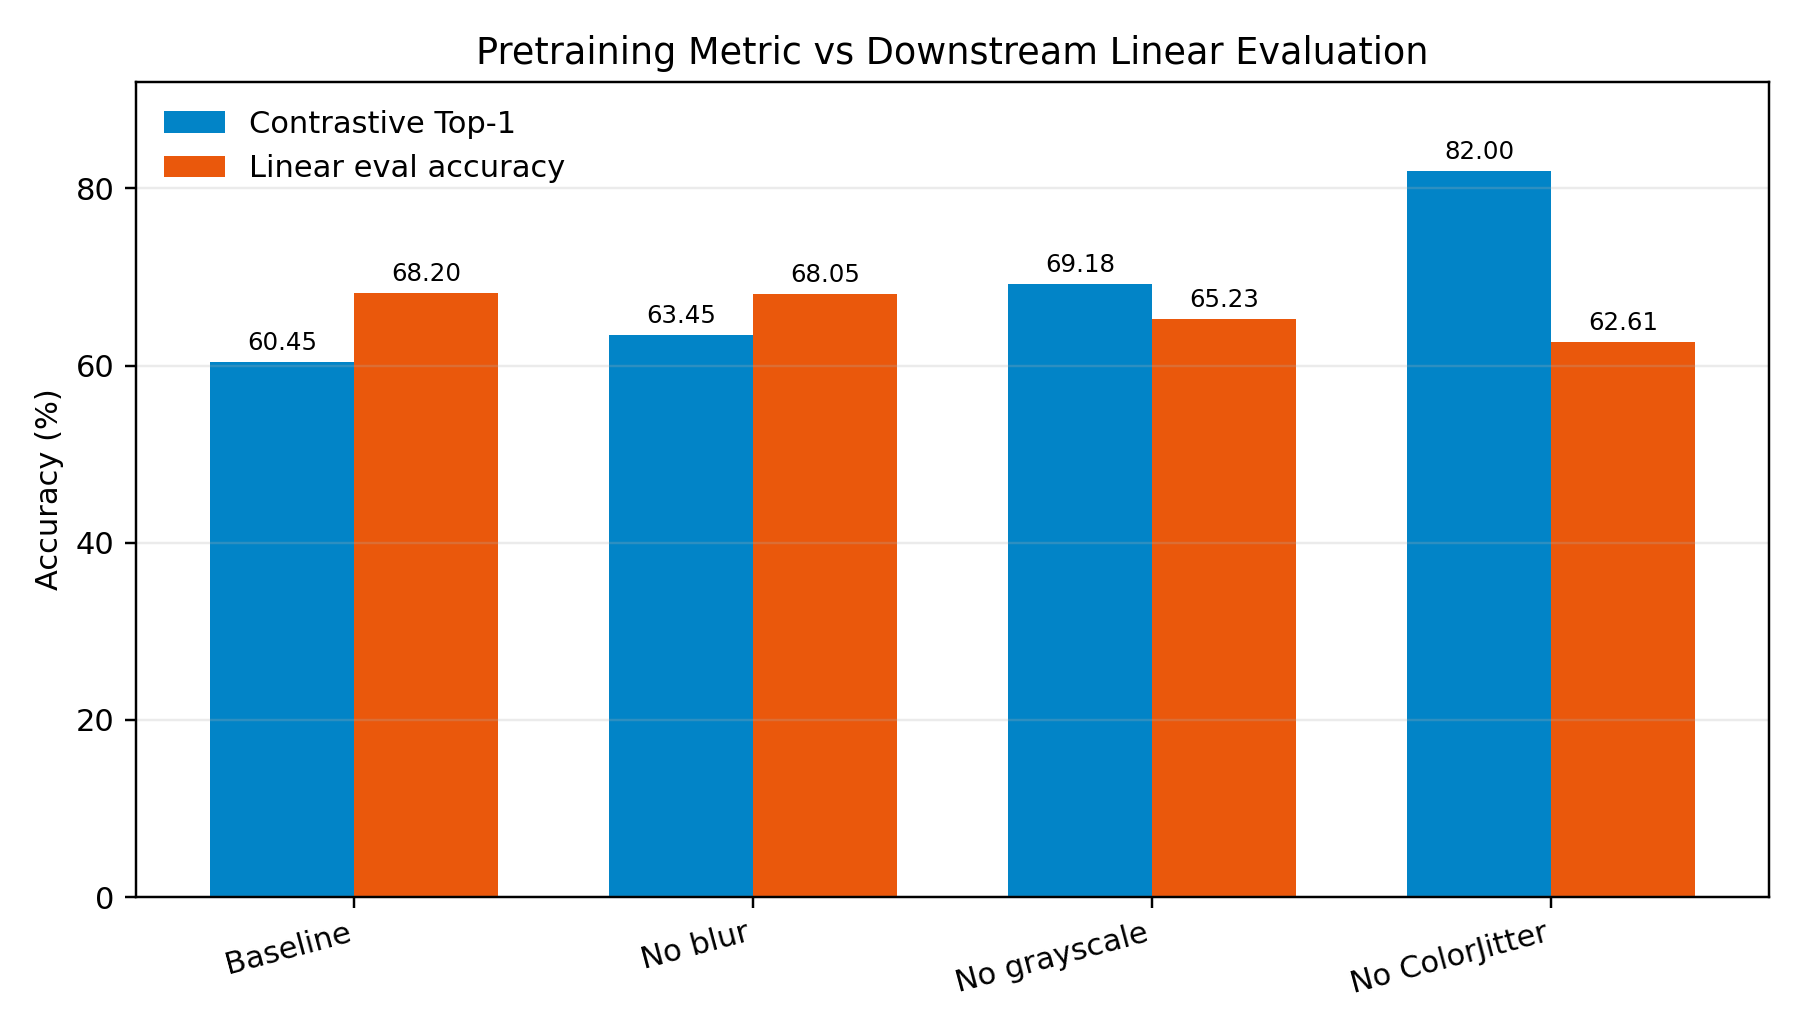
\includegraphics[width=0.70\textwidth]{augmentation_figures/augmentation_metrics_bar.png}
\caption{Visualization of the data augmentation ablation results.}
\label{fig:augmentation-visualization}
\end{figure}

The baseline obtains the best downstream accuracy, reaching 68.20\%. Removing Gaussian blur gives a very similar result, 68.05\%. Removing random grayscale causes a larger drop to 65.23\%. The largest drop comes from removing ColorJitter, which reduces accuracy to 62.61\%. This suggests that ColorJitter is the most important augmentation among the three tested data augmentation methods.

The contrastive Top-1 metric does not match the downstream ranking. The no\_color\_jitter setting achieves the highest contrastive Top-1 score, 82.00, but gives the worst frozen linear evaluation accuracy. Therefore, we use frozen linear evaluation as the main measure of representation quality.

\subsection{Projection Head Ablation}

In this experiment, the intended variable is whether the model uses the projection head during SimCLR pretraining. Other settings are kept the same within this experiment, including CIFAR-10, ResNet-18, and 100-epoch pretraining checkpoint.

\begin{table}[H]
\centering
\small
\begin{tabular}{lccc}
\toprule
\textbf{Setting} & \textbf{Encoder dim.} & \textbf{Best acc. (\%)} & \textbf{Final acc. (\%)} \\
\midrule
With projection head & 512 & \textbf{63.59} & \textbf{62.84} \\
Without projection head & 512 & 62.16 & 61.40 \\
\bottomrule
\end{tabular}
\caption{Linear evaluation result for the projection head ablation.}
\label{tab:projection-head}
\end{table}

\begin{figure}[H]
\centering
\begin{subfigure}{0.45\textwidth}
    \centering
    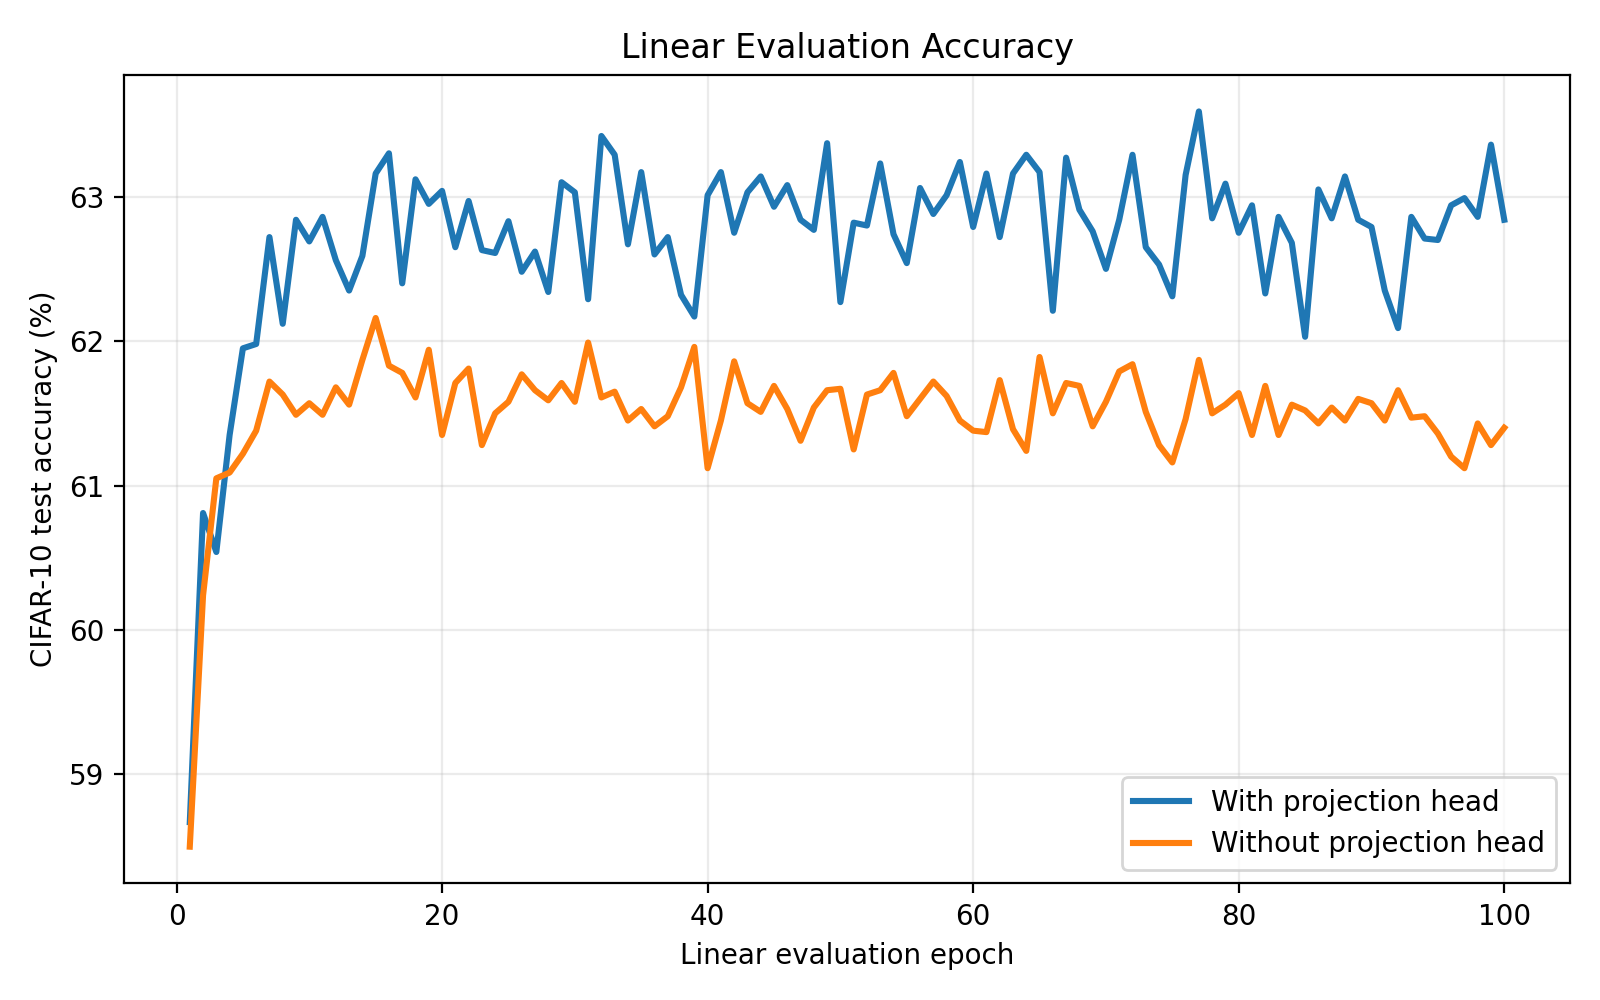
\includegraphics[width=\textwidth]{head_figures/accuracy_curve.png}
    \caption{Linear-evaluation accuracy.}
\end{subfigure}
\hfill
\begin{subfigure}{0.45\textwidth}
    \centering
    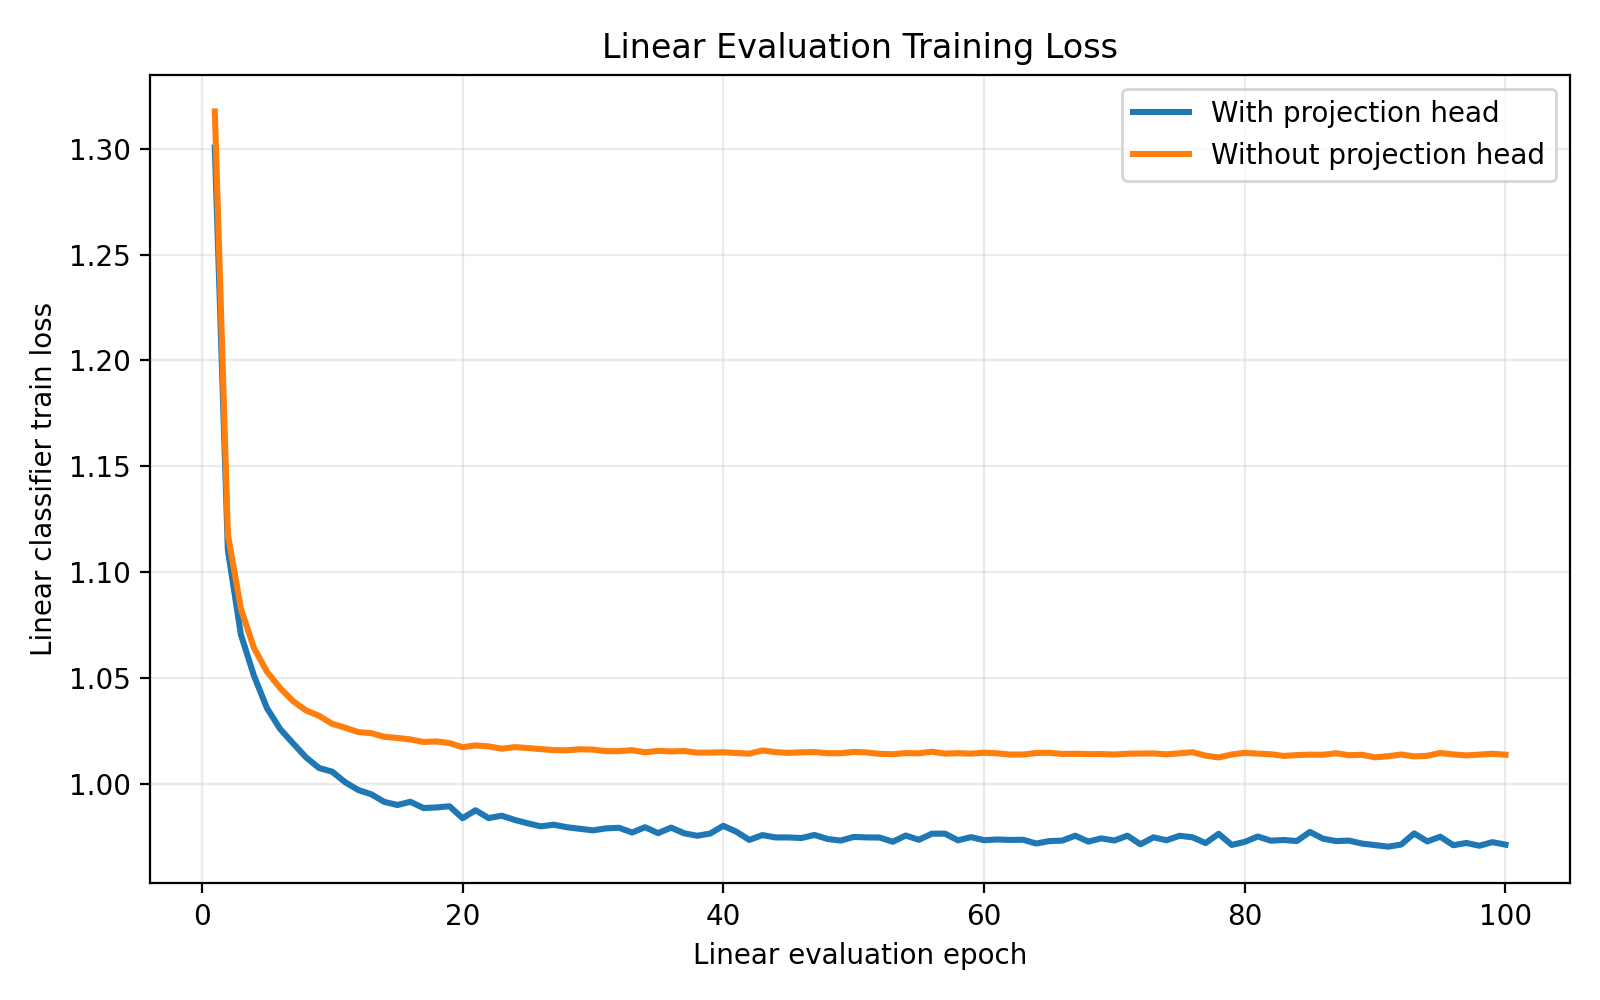
\includegraphics[width=\textwidth]{head_figures/loss_curve.png}
    \caption{Linear-evaluation loss.}
\end{subfigure}
\caption{Projection head ablation curves.}
\label{fig:projection-head}
\end{figure}

The model with the projection head reaches 63.59\% best test accuracy, while the model without the projection head gets 62.16\%. The final accuracy also improves from 61.40\% to 62.84\%. This supports the SimCLR design that applies the contrastive loss in the projected space $z$, while downstream evaluation uses the encoder feature $h$.

One possible explanation is that the projection head helps separate contrastive learning from the final representation used for classification. The contrastive loss encourages positive pairs to be similar and negative pairs to be different. If this objective is applied directly to $h$, some useful information for classification may be lost. The projection head allows $z$ to focus on the contrastive task, while $h$ keeps more useful visual features for downstream tasks.

\subsection{Batch Size Ablation}
\label{sec:batch-size}

Batch size changes the number of negatives in the contrastive loss. With two views per image, the number of negatives for each anchor is $2B-2$. We compare batch sizes 128, 256, 512, and 1024 within the same batch-size experiment. The projection head is enabled for this ablation, and the same linear evaluation protocol is used for all four runs.

\begin{table}[H]
\centering
\small
\begin{tabular}{ccccc}
\toprule
\textbf{Batch size} & \textbf{Negatives/anchor} & \textbf{Best acc. (\%)} & \textbf{Best epoch} & \textbf{Final acc. (\%)} \\
\midrule
128 & 254 & 62.54 & 49 & 62.10 \\
256 & 510 & \textbf{63.47} & 29 & \textbf{63.33} \\
512 & 1022 & 60.89 & 45 & 60.29 \\
1024 & 2046 & 57.56 & 64 & 56.88 \\
\bottomrule
\end{tabular}
\caption{Linear evaluation result for the batch size ablation.}
\label{tab:batch-size}
\end{table}

\begin{figure}[H]
\centering
\begin{subfigure}{0.45\textwidth}
    \centering
    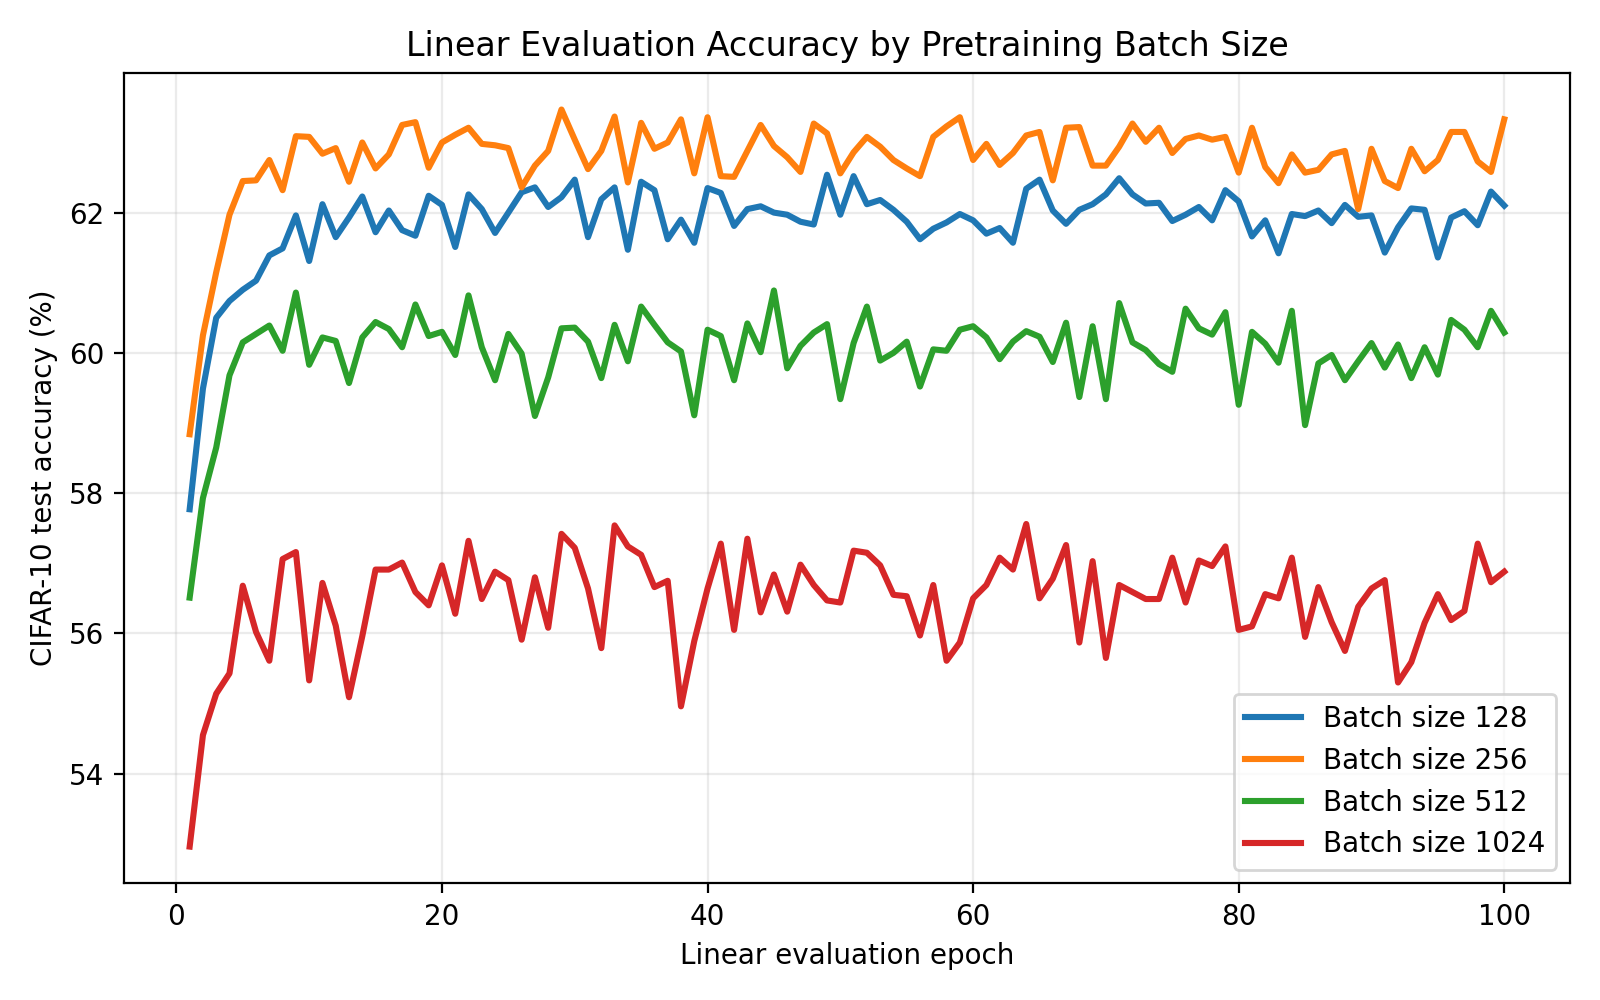
\includegraphics[width=\textwidth]{batch_figures/accuracy_curve.png}
    \caption{Linear-evaluation accuracy over epochs.}
\end{subfigure}
\hfill
\begin{subfigure}{0.45\textwidth}
    \centering
    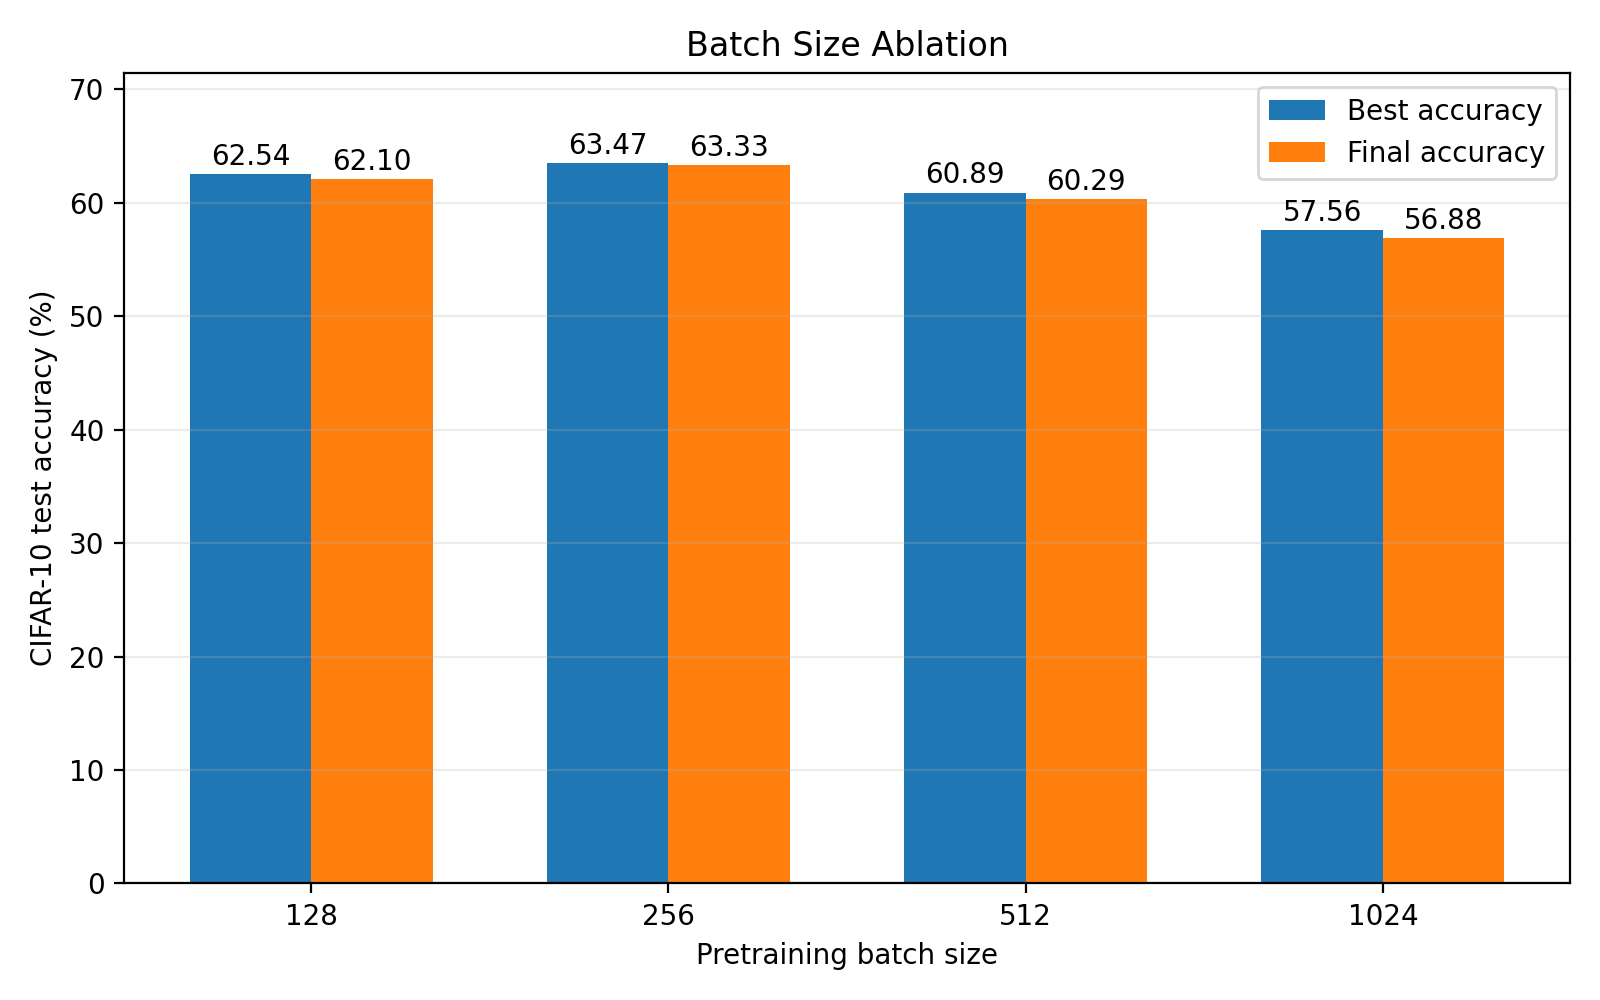
\includegraphics[width=\textwidth]{batch_figures/accuracy_bar.png}
    \caption{Best and final test accuracy.}
\end{subfigure}
\caption{Batch size ablation results.}
\label{fig:batch-size}
\end{figure}

The best result is obtained at batch size 256, with 510 negatives per anchor and 63.47\% best test accuracy. Batch size 128 is slightly lower at 62.54\%, while batch sizes 512 and 1024 drop to 60.89\% and 57.56\%, respectively. Therefore, our result does not show a monotonic improvement from using more negative samples.

Large batch size changes more than the number of negatives. It also changes the number of optimizer updates per epoch, the probability of false negatives, and the match between learning rate and batch size. We discuss these factors in Section~\ref{sec:discussion}. To further test whether the weak batch size 1024 result is caused by large batches themselves or by optimization mismatch, we conduct a learning-rate follow-up experiment in Section~\ref{sec:lr-followup}.

\subsection{Low-Label Evaluation}

This experiment tests whether SimCLR representations are useful when only a small number of labels are available. We use two evaluation settings. First, in frozen linear evaluation, the SimCLR encoder is frozen and only the linear classifier is trained using a subset of labels. This measures the quality of the pretrained feature space. Second, in non-frozen transfer, the whole model is trained with labels, and we compare SimCLR initialization against supervised training from scratch.

\begin{table}[H]
\centering
\small
\begin{tabular}{lccccc}
\toprule
\textbf{Evaluation setting} & \textbf{1\%} & \textbf{10\%} & \textbf{50\%} & \textbf{80\%} & \textbf{100\%} \\
\midrule
Frozen SimCLR + linear classifier & 54.3 & 64.4 & 67.2 & 67.7 & \textbf{68.2} \\
\bottomrule
\end{tabular}
\caption{Frozen linear evaluation accuracy under different label fractions. Only linear classifier is trained.}
\label{tab:low-label-frozen}
\end{table}

The frozen SimCLR features remain useful even when labels are limited. With only 1\% of labels, the linear classifier reaches 54.3\% accuracy. With 10\% of labels, it reaches 64.4\%, which is only 3.8 percentage points below the 100\% label result. This indicates that the pretrained encoder has already learned a useful dataset feature space before supervised labels are used.

\begin{table}[H]
\centering
\small
\begin{tabular}{lccc}
\toprule
\textbf{Method} & \textbf{1\% labels} & \textbf{10\% labels} & \textbf{100\% labels} \\
\midrule
Supervised from scratch & 34.3 & 55.7 & 76.4 \\
SimCLR initialization + fine-tuning & \textbf{54.3} & \textbf{66.7} & \textbf{78.4} \\
\bottomrule
\end{tabular}
\caption{Non-frozen transfer comparison. Both methods train the encoder and classifier with labels, but use different initializations.}
\label{tab:low-label-transfer}
\end{table}

\begin{figure}[H]
\centering
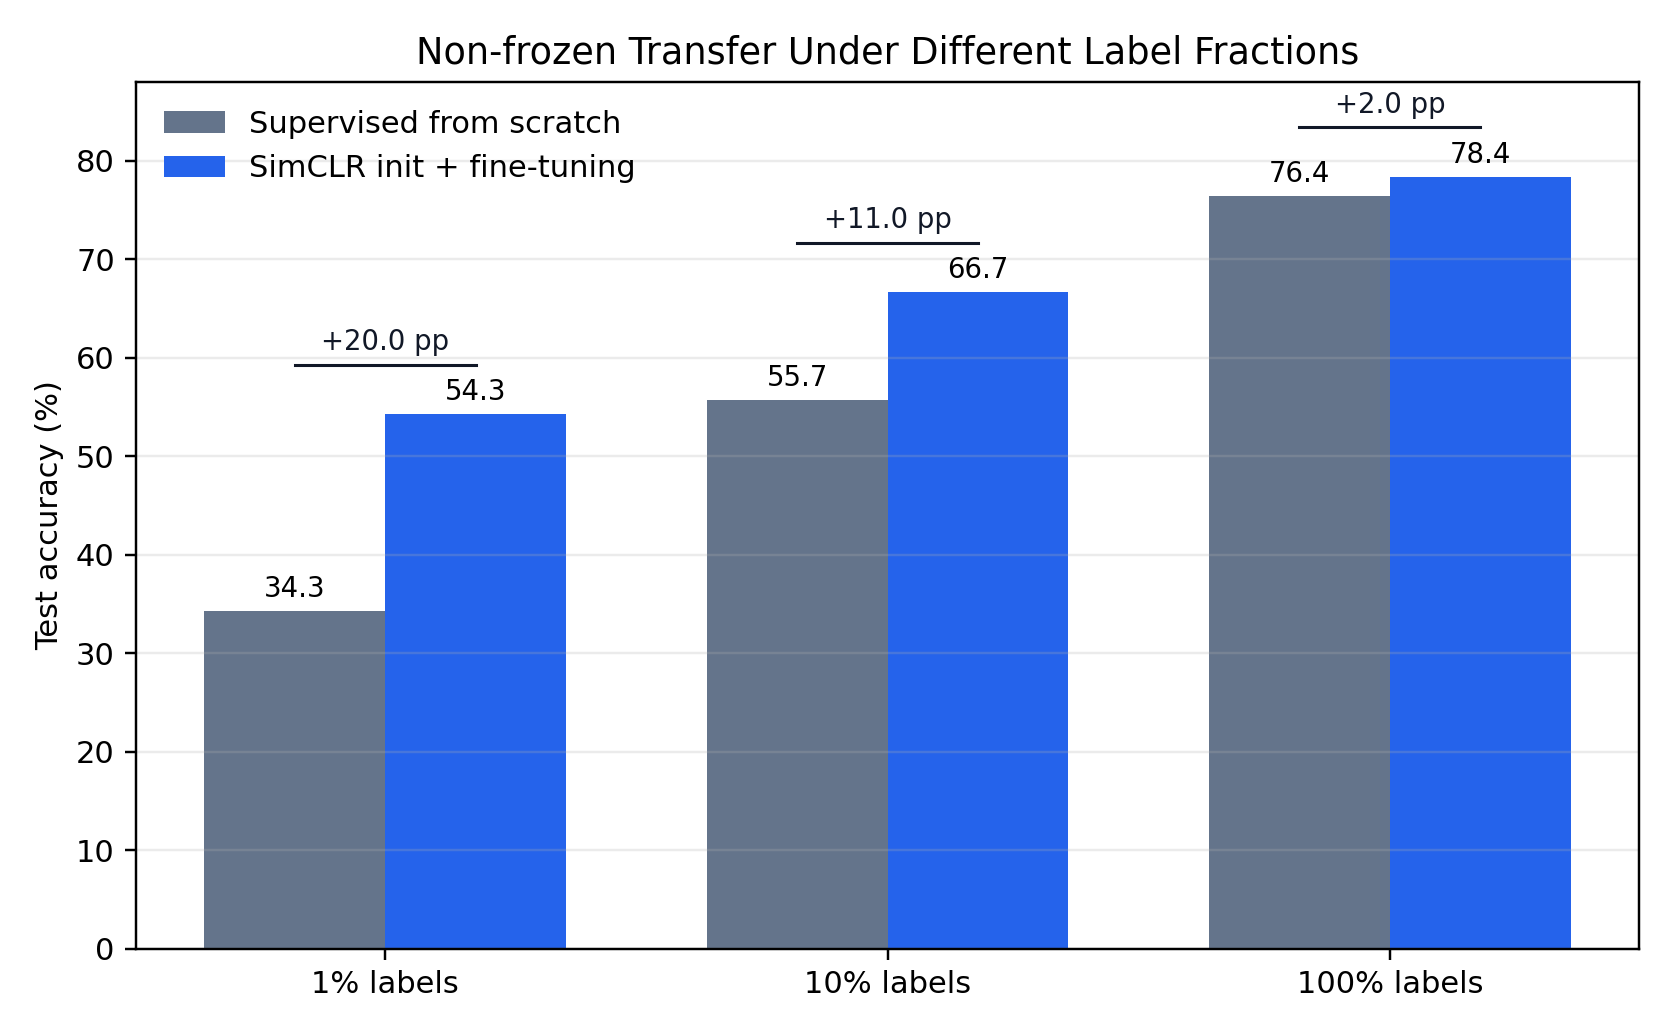
\includegraphics[width=0.70\textwidth]{low_label_figures/low_label_transfer_accuracy.png}
\caption{Non-frozen transfer accuracy under different label fractions.}
\label{fig:low-label-transfer}
\end{figure}

The advantage of SimCLR is largest when labels are scarce. At 1\% labels, SimCLR initialization improves accuracy from 34.3\% to 54.3\%, a gain of 20.0 percentage points. At 10\% labels, the gain is 11.0 percentage points. With all labels, the gain shrinks to 2.0 percentage points. This shows that SimCLR mainly improves label efficiency: it is most helpful when supervised labels are limited, and its advantage becomes smaller as more labels become available.

\subsection{Large-Batch Learning Rate Follow-up}
\label{sec:lr-followup}

The batch size ablation in Section~\ref{sec:batch-size} shows that batch size 1024 performs poorly under the default learning rate. This follow-up experiment checks whether the weak large-batch result is partly an optimization issue. We keep the batch size fixed at 1024 and sweep the pretraining learning rate. The default learning rate is too small for this large-batch setting, but increasing it too far also hurts performance.

\begin{table}[H]
\centering
\small
\begin{tabular}{lcc}
\toprule
\textbf{Learning rate} & \textbf{Best acc. (\%)} & \textbf{Change from default} \\
\midrule
$3 \times 10^{-4}$ & 57.56 & -- \\
$6 \times 10^{-4}$ & 63.73 & +6.17 \\
$1.2 \times 10^{-3}$ & \textbf{65.43} & +7.87 \\
$2.4 \times 10^{-3}$ & 61.22 & +3.66 \\
\bottomrule
\end{tabular}
\caption{Learning-rate sweep for batch size 1024.}
\label{tab:large-batch-lr}
\end{table}

\begin{figure}[H]
\centering
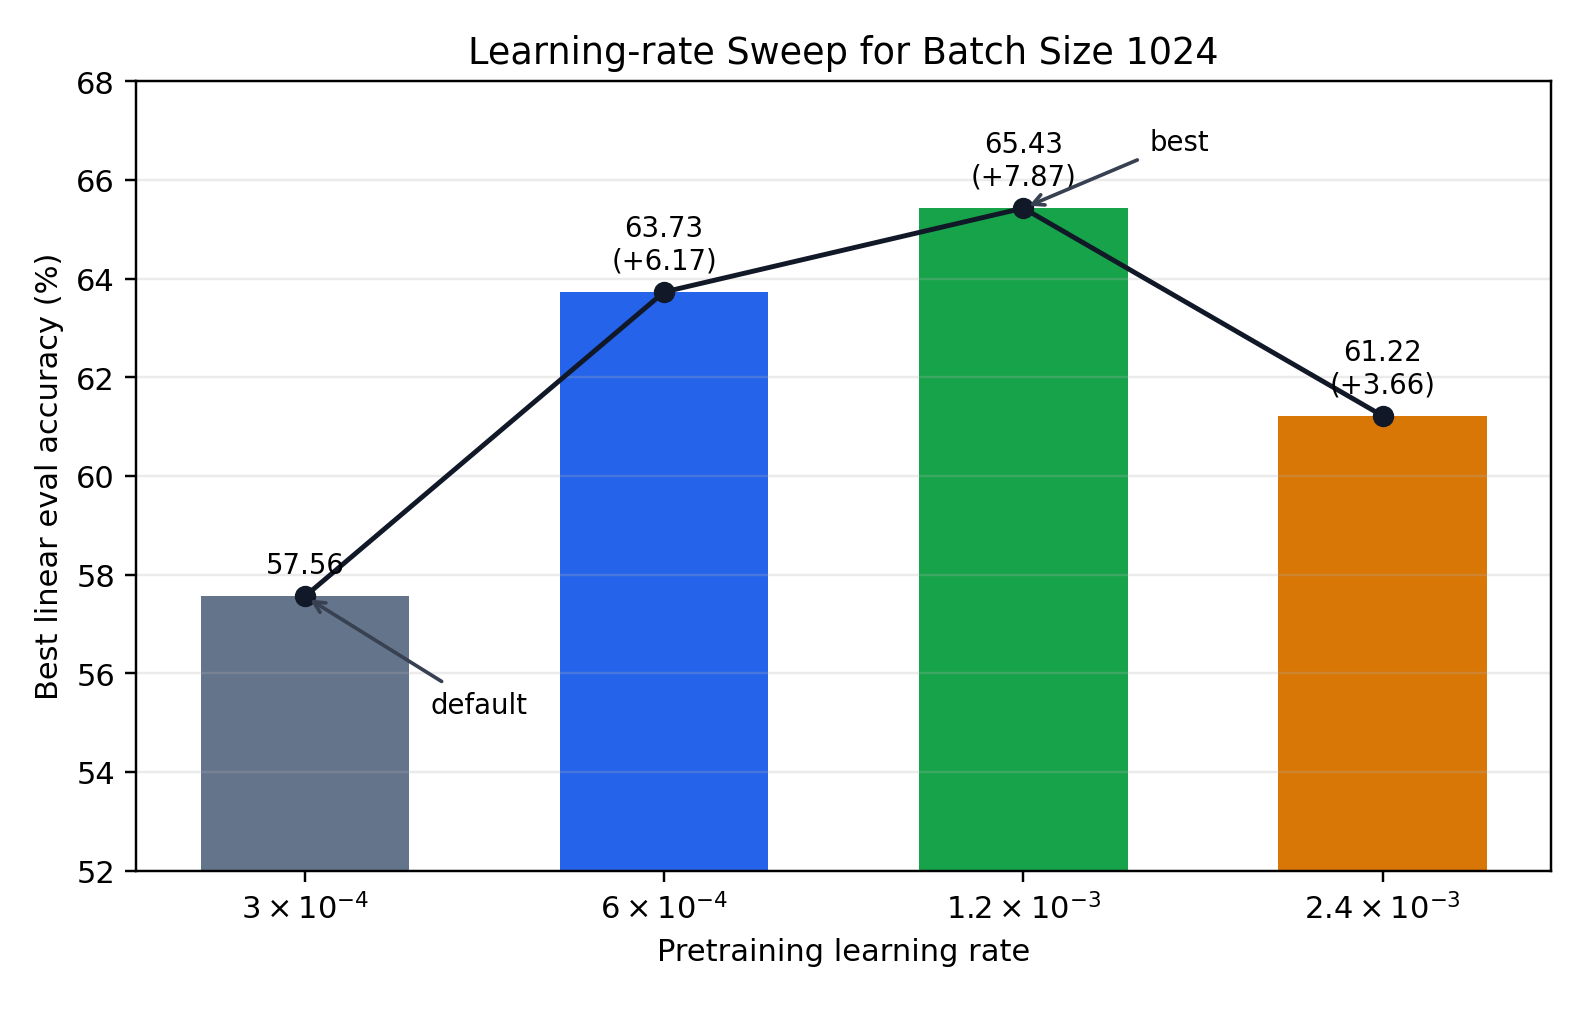
\includegraphics[width=0.70\textwidth]{lr_figures/large_batch_lr_sweep.png}
\caption{Learning-rate sweep for batch size 1024.}
\label{fig:large-batch-lr}
\end{figure}

The best result is obtained with learning rate $1.2 \times 10^{-3}$, which improves the batch size 1024 result from 57.56\% to 65.43\%. This changes how we interpret the batch size ablation. The weak default result for batch size 1024 does not mean that more negatives are always harmful. Instead, it suggests that large-batch SimCLR needs a matched optimization setting. With a fixed number of epochs, a larger batch gives fewer optimizer updates per epoch, so the default learning rate may not make enough progress. However, the result at $2.4 \times 10^{-3}$ also shows that a larger learning rate is not monotonically better.

\section{Discussions}
\label{sec:discussion}

Overall, the experiments show that SimCLR performance is affected by both representation design and optimization detials. Data augmentation and projection head mainly affect what information is encouraged in the representation, while batch size and learning rate affect how well the contrastive objective is optimized.

\textbf{Data Augmentation: }The data augmentation ablation shows that ColorJitter is the most important augmentation in our baseline setting. Removing ColorJitter leads to the largest drop in downstream accuracy, even though it achieves the highest contrastive Top-1 score. One possible reason is that without ColorJitter, two views of the same image keep similar color information. The model then rely on these simple color cues to solve contrastive task instead of learning more useful features like object shapes and structures. 

In contrast, removing Gaussian blur has almost no negative effect. One possible reason is that CIFAR-10 images are very small ($32 \times 32$ pixels), so blur may remove too much image detail. In addition, CIFAR-10 classification may depend more on overall object shapes than on fine textures. As a result, removing blur does not highly reduce representation quality in our experiments. Overall, frozen linear evaluation provides a more reliable measure of representation quality than contrastive Top-1 accuracy.

\textbf{Projection Head: }The projection head ablation shows that applying the contrastive loss in a projected space improves the final representation. The downstream classifier uses $h$, while NT-Xent directly optimizes $z$. This separation is useful because NT-Xent encourages positive-pair alignment while also spreading negative samples more uniformly across the representation space. The projection head can therefore act as an information filter: $z$ focuses more on the contrastive task, while $h$ keeps more general visual information for downstream classification.

\textbf{Batch Size and Optimization: }The batch size ablation gives a more mixed result than the original SimCLR trend. With the default learning rate, batch size 256 performs best, while 512 and 1024 perform worse. This does not mean that more negative samples are unhelpful. Batch size affects several factors at once, including the number of negatives, optimization behavior, false negatives, and learning-rate settings.

The false-negative issue is especially important for CIFAR-10 because it contains only ten classes. In a large batch, many negative samples may actually belong to the same class as the anchor image. SimCLR still treats these samples as negatives, forcing them apart in the representation space. This can reduce similarity between same-class samples and make it harder to form clear semantic clusters.

The learning-rate experiment helps explain the large-batch results. For batch size 1024, accuracy increases from 57.56\% to 65.43\% when the learning rate is increased to $1.2 \times 10^{-3}$. This suggests that the poor default result is partly caused by optimization issues. However, the result at $2.4 \times 10^{-3}$ drops again, so large-batch SimCLR needs matched optimization, not just more negatives.

\textbf{Low-Label Transfer: }The low-label evaluation shows the practical value of SimCLR. In frozen evaluation, 10\% labels gives 64.4\% accuracy, only 3.8 percentage points below the full-label result. In non-frozen transfer, SimCLR initialization gives the largest gain at 1\% labels. This suggests that the main benefit of SimCLR is label efficiency rather than simply improving the fully supervised setting.

\section{Shortcomings}

There are several limitations in the current experiments. First, although some settings were checked with repeated 100-epoch evaluation runs, we do not report full mean and standard deviation for every setting. Therefore, small differences, such as 68.20\% versus 68.05\%, should not be over-interpreted. Our main conclusions rely on larger trends, such as the drop caused by removing ColorJitter, the recovery of batch size 1024 after learning-rate tuning, and the low-label gains from SimCLR initialization. Second, when best accuracy is reported, it refers to the highest test accuracy observed during the corresponding 100-epoch linear evaluation, rather than a complete statistical estimate over many random seeds. Besides, the experiments use CIFAR-10 and ResNet-18 only, so the conclusions may not transfer directly to larger datasets or architectures. Finally, some comparisons use the same number of epochs rather than the same number of optimization steps, which can disadvantage larger batches.

\section{Future Work}

Future work could run each setting with multiple random seeds and report mean and standard deviation. The batch size ablation could also be extended with learning-rate scaling, longer pretraining, LARS or SGD with momentum, temperature tuning, and schedules matched by number of optimization steps rather than only by epochs. Finally, k-nearest-neighbor evaluation and feature-space visualization could be added to better understand how different ablations change the learned representation space.

\section{Conclusion}

This project presents an ablation study of SimCLR on CIFAR-10 using a ResNet-18 encoder. Removing ColorJitter causes the largest drop in downstream accuracy, even though it achieves the highest contrastive Top-1 score, showing that pretraining metrics do not always reflect representation quality. The projection head improves best linear evaluation accuracy from 62.16\% to 63.59\%, showing the benefit of learning in a separate projected space. In the batch size experiments, batch size 256 performs best under the default settings, but batch size 1024 improves to 65.43\% when the learning rate is matched. Finally, the low-label experiments show that SimCLR mainly improves label efficiency, with the largest gain at 1\% labels. Overall, SimCLR works well in our lightweight setting, and its performance is strongly affected by data augmentation, projection head design, and optimization matching.


\begin{thebibliography}{10}

\bibitem{simclr}
T. Chen, S. Kornblith, M. Norouzi, and G. Hinton.
\textit{A Simple Framework for Contrastive Learning of Visual Representations}.
ICML, 2020.
\url{https://arxiv.org/abs/2002.05709}

\bibitem{cpc}
A. van den Oord, Y. Li, and O. Vinyals.
\textit{Representation Learning with Contrastive Predictive Coding}.
arXiv preprint arXiv:1807.03748, 2018.
\url{https://arxiv.org/abs/1807.03748}

\bibitem{moco}
K. He, H. Fan, Y. Wu, S. Xie, and R. Girshick.
\textit{Momentum Contrast for Unsupervised Visual Representation Learning}.
CVPR, 2020.
\url{https://arxiv.org/abs/1911.05722}

\bibitem{simclrv2}
T. Chen, S. Kornblith, K. Swersky, M. Norouzi, and G. Hinton.
\textit{Big Self-Supervised Models are Strong Semi-Supervised Learners}.
NeurIPS, 2020.
\url{https://arxiv.org/abs/2006.10029}

\bibitem{supcon}
P. Khosla, P. Teterwak, C. Wang, A. Sarna, Y. Tian, P. Isola, A. Maschinot, C. Liu, and D. Krishnan.
\textit{Supervised Contrastive Learning}.
NeurIPS, 2020.
\url{https://arxiv.org/abs/2004.11362}

\bibitem{byol}
J.-B. Grill, F. Strub, F. Altch'e, C. Tallec, P. Richemond, E. Buchatskaya, C. Doersch, B. Avila Pires, Z. Guo, M. G. Azar, B. Piot, K. Kavukcuoglu, R. Munos, and M. Valko.
\textit{Bootstrap Your Own Latent: A New Approach to Self-Supervised Learning}.
NeurIPS, 2020.
\url{https://arxiv.org/abs/2006.07733}

\bibitem{simsiam}
X. Chen and K. He.
\textit{Exploring Simple Siamese Representation Learning}.
CVPR, 2021.
\url{https://arxiv.org/abs/2011.10566}

\bibitem{cifar10}
A. Krizhevsky.
\textit{Learning Multiple Layers of Features from Tiny Images}.
Technical report, 2009.
\url{https://www.cs.toronto.edu/~kriz/cifar.html}

\bibitem{resnet}
K. He, X. Zhang, S. Ren, and J. Sun.
\textit{Deep Residual Learning for Image Recognition}.
CVPR, 2016.
\url{https://arxiv.org/abs/1512.03385}

\end{thebibliography}


\end{document}
